\documentclass[conference]{IEEEtran}

\usepackage[T1]{fontenc}
\usepackage[utf8]{inputenc}
\usepackage{amsmath,amssymb}
\usepackage{graphicx}
\usepackage{subcaption}
\usepackage{booktabs}
\usepackage{siunitx}
\usepackage{url}
\usepackage[hidelinks]{hyperref}
% Sin esto, url usa Courier en T1 (pcrr8t) y pdflatex lo genera como bitmap:
% es el 'mktextfm pcrr8t' que aparece en missfont.log.
\urlstyle{same}

\sisetup{separate-uncertainty=true,detect-all=true}
\graphicspath{{img/}}

\begin{document}

\title{Aberration Analysis of Reflecting and Refracting\\
Optical Systems}

\author{\IEEEauthorblockN{Nicol\'as Seguel}
\IEEEauthorblockA{Laboratorio de Instrumentación Astronómica -- IEE3873\\
Pontificia Universidad Cat\'olica de Chile\\
\texttt{neseguel@uc.cl}}}

\maketitle

\section{Introduction}

The purpose of this laboratory is to use optical design software, ATMOS
\cite{atmos} and Zemax OpticStudio, to measure how the image quality of a
system depends on its geometry. Three families are traced: single mirrors,
spherical and parabolic, over a range of focal ratios; the classical
two-mirror telescopes; and singlet lenses.

Each configuration is judged with the same three tools: the aberration
curves, which say what is wrong with the wavefront; the spot diagram, which
says how large the image of a point source is; and the modulation transfer
function, which says how much contrast survives at each spatial frequency.

\section{Theoretical Framework}
\label{sec:theory}

\subsection{Aberrations}

The wavefront aberration $W$ is the departure of the real wavefront from a
sphere centred on the image point, measured in waves. Rays travel normal to
the wavefront, so the transverse ray aberration $\varepsilon$, the distance
between where a ray lands and where the paraxial ray lands, is proportional to
the slope of $W$ \cite{guide}. Ray fans plot $\varepsilon$ and OPD fans plot
$W$; both describe the same defect.

To third order each aberration carries its own power of the normalized pupil
radius $r$ and field height $\beta$: spherical aberration goes as $r^4$ and
does not depend on the field, coma as $\beta r^3$, and astigmatism as
$\beta^2r^2$. For a mirror of diameter $D$ and radius $R = 2f$ at infinite
conjugate, the transverse spherical aberration of a sphere and the
peak-to-valley wavefront error at best focus are
\begin{equation}
\mathrm{TSA} = \frac{D}{64N^2},
\qquad
W_{PV} = \frac{D}{2048\,N^3},
\label{eq:sa}
\end{equation}
with $N = f/D$ the focal ratio; both vanish for a paraboloid, $K = -1$. Coma
does not depend on the conic constant when the stop is on the mirror, and is
measured by the offence against the sine condition
\begin{equation}
\mathrm{OSC} = \frac{1}{16N^2},
\label{eq:osc}
\end{equation}
which becomes a linear blur through $\mathrm{Coma}_{tan} = 3\,\mathrm{OSC}\,h'$
with $h' = f\tan\theta$ the image height.

\subsection{Spot diagram}

The spot diagram is the set of intercepts in the image plane of rays
uniformly sampling the pupil. It is purely geometrical, so it is meaningful
only against the size diffraction imposes even on a perfect system, the Airy
disc,
\begin{equation}
d_{\mathrm{Airy}} = 2.44\,\lambda N.
\label{eq:airy}
\end{equation}
A system whose spot fits inside the Airy disc is diffraction limited. Since
$d_{\mathrm{Airy}}$ grows with $N$, configurations are compared through the
ratio between the RMS spot radius and the Airy radius, not the spot size
alone.

\subsection{Modulation transfer function}

The MTF is the contrast transferred as a function of spatial frequency, and
is the modulus of the Fourier transform of the point spread function. An
aberration-free system has an MTF limited only by diffraction, falling
monotonically to zero at
\begin{equation}
\nu_c = \frac{1}{\lambda N}.
\label{eq:cutoff}
\end{equation}
Aberrations depress the curve below that ideal. A strongly aberrated system
can show the curve reaching zero and rising again, which is spurious
resolution: contrast returns with the fringes reversed.

\section{Equipment and Method}
\label{sec:equip}

\begin{table}[htbp]
\caption{Tools used in the analysis.}
\label{tab:equip}
\centering
\small
\begin{tabular}{@{}ll@{}}
\toprule
\textbf{Item} & \textbf{Use} \\
\midrule
Zemax OpticStudio & ray tracing, spot diagrams, MTF \\
ATMOS v8.96 & cross-check of aberration coefficients \\
Personal computer & simulation and data reduction \\
Schott glass catalogue & refractive indices of the lenses \\
\bottomrule
\end{tabular}
\end{table}

All systems use the same aperture, $D = \SI{200}{\milli\meter}$, so that the
spot diagrams of different configurations are directly comparable. The
reference wavelength is \SI{550}{\nano\meter} for the mirror systems, which
are achromatic by construction; the lenses are evaluated at 450, 550 and
\SI{650}{\nano\meter}. The stop is on the first optical surface of every
system. The single mirrors are sampled at $0$, $0.5$, $1$ and
\SI{2}{\degree}, the telescopes at $0$, $0.25$ and \SI{0.5}{\degree}.

The four telescopes share a primary of $f/3$ ($R_1 = \SI{-1200}{\milli\meter}$)
and a secondary magnification $m = 5$, giving $f/15$ and an effective focal
length of \SI{3000}{\milli\meter}. The Newtonian instead uses a single
$f/15$ paraboloid, $R = \SI{-6000}{\milli\meter}$. The conic constants and
secondary radii follow from the design family, as listed in
Table~\ref{tab:telprescription}.

\section{Results}
\label{sec:res}

\subsection{Spherical and parabolic mirrors}
\label{sec:res-mirrors}

Table~\ref{tab:mirrors} collects the spot data. On axis the spherical mirror
reproduces \eqref{eq:sa} closely: the measured geometrical radius is
\SI{511.5}{\micro\meter} at $f/2.5$ against the \SI{500}{\micro\meter}
predicted, and \SI{7.82}{\micro\meter} at $f/20$ against \SI{7.81}{}. The
agreement improves from \SI{2.3}{\percent} to \SI{0.06}{\percent} as $N$
grows, which is the higher-order content of the aberration disappearing.

The spherical mirror stops being the dominant defect near $f/15$: there the
on-axis RMS radius, \SI{7.96}{\micro\meter}, falls below the Airy radius of
\SI{10.07}{\micro\meter}, and at $f/20$ the whole geometrical spot fits
inside the Airy disc. Figures~\ref{fig:sph25} and \ref{fig:sph20} show the
same mirror at the two extremes.

The paraboloid gives an on-axis RMS radius of zero at every focal ratio
(Fig.~\ref{fig:par25}). Off axis it is no better than the sphere: at
\SI{0.5}{\degree} its RMS radius falls as $1/N$, from \SI{56.1}{\micro\meter}
at $f/2.5$ to \SI{7.40}{\micro\meter} at $f/20$, which is the scaling of
\eqref{eq:osc} at fixed field angle.

\begin{table}[htbp]
\caption{Single mirrors of \SI{200}{\milli\meter} aperture. Radii in
\si{\micro\meter}, from the Zemax spot diagrams.}
\label{tab:mirrors}
\centering
\small
\begin{tabular}{@{}lcccc@{}}
\toprule
$N$ & Airy rad. & RMS $0^\circ$ & GEO $0^\circ$ & RMS \SI{0.5}{\degree} \\
\midrule
\multicolumn{5}{@{}l}{\emph{Spherical, $K=0$}} \\
2.5 & 1.686  & 201.900 & 511.486 & 256.190 \\
5   & 3.350  & 71.913  & 125.707 & 68.110 \\
10  & 6.712  & 17.912  & 31.294  & 21.985 \\
15  & 10.066 & 7.956   & 13.895  & 13.054 \\
20  & 13.421 & 4.474   & 7.815   & 9.630 \\
\midrule
\multicolumn{5}{@{}l}{\emph{Parabolic, $K=-1$}} \\
2.5 & 1.604  & 0.000 & 0.000 & 56.119 \\
5   & 3.363  & 0.000 & 0.000 & 28.119 \\
10  & 6.714  & 0.000 & 0.000 & 14.470 \\
15  & 10.068 & 0.000 & 0.000 & 10.087 \\
20  & 13.422 & 0.000 & 0.000 & 7.398 \\
\bottomrule
\end{tabular}
\end{table}

\begin{figure*}[tbp]
\centering
\includegraphics[width=\textwidth]{{01/sphere_2.5_report}.jpg}
\caption{Spherical mirror at $f/2.5$: layout, transverse ray fan, spot
diagram and polychromatic diffraction MTF. The ray fan shows the cubic
signature of spherical aberration and the MTF collapses within a few tens of
cycles per millimetre.}
\label{fig:sph25}
\end{figure*}

\begin{figure*}[tbp]
\centering
\includegraphics[width=\textwidth]{{01/conic_2.5_report}.jpg}
\caption{Parabolic mirror at $f/2.5$. The on-axis spot collapses to a point
and the on-axis MTF follows the ideal curve; the off-axis fields keep the
coma that the conic constant cannot remove.}
\label{fig:par25}
\end{figure*}

\begin{figure*}[tbp]
\centering
\includegraphics[width=\textwidth]{{01/sphere_20_report}.jpg}
\caption{Spherical mirror at $f/20$. The geometrical spot now fits inside the
Airy disc and the MTF approaches the diffraction limit, so at this focal
ratio the sphere behaves as a perfect surface.}
\label{fig:sph20}
\end{figure*}

\subsection{Two-mirror telescopes}
\label{sec:res-tel}

All four designs null spherical aberration on axis: the RMS radius is below
\SI{0.01}{\micro\meter} in every case (Table~\ref{tab:telperf}), which
confirms the conic constants of Table~\ref{tab:telprescription}. The
differences appear entirely in the field.

At \SI{0.5}{\degree} the Newtonian gives \SI{11.6}{\micro\meter}, the
Gregorian \SI{48.6}{}, the Ritchey-Chr\'etien \SI{64.6}{} and the classical
Cassegrain \SI{63.4}{}, against an Airy radius of \SI{10.07}{\micro\meter}.
The Cassegrain and the Ritchey-Chr\'etien are indistinguishable in RMS, but
their maximum radii differ, \SI{115.1}{} against \SI{96.8}{\micro\meter}.
Fig.~\ref{fig:cass} shows the Cassegrain spot diagrams.

\begin{table}[htbp]
\caption{Prescriptions of the four telescopes, all \SI{200}{\milli\meter} and
$f/15$.}
\label{tab:telprescription}
\centering
\small
\begin{tabular}{@{}lccccc@{}}
\toprule
\textbf{Design} & $R_1$ & $K_1$ & $R_2$ & $K_2$ & Obstr. \\
 & [mm] & & [mm] & & [\%] \\
\midrule
Newtonian            & $-6000$ & $-1$ & --- & --- & 7.5 \\
Classical Cassegrain & $-1200$ & $-1$ & $-333.33$ & $-2.2500$ & 22.2 \\
Gregorian            & $-1200$ & $-1$ & $+333.33$ & $-0.4444$ & 33.3 \\
Ritchey-Chr\'etien   & $-1200$ & $-1.0234$ & $-333.33$ & $-2.4561$ & 22.2 \\
\bottomrule
\end{tabular}
\end{table}

\begin{table}[htbp]
\caption{RMS spot radius of the telescopes against field angle, in
\si{\micro\meter}. The Airy radius at $f/15$ is \SI{10.07}{\micro\meter}.}
\label{tab:telperf}
\centering
\small
\begin{tabular}{@{}lcccc@{}}
\toprule
\textbf{Design} & $0^\circ$ & \SI{0.25}{\degree} & \SI{0.5}{\degree} &
Max \SI{0.5}{\degree} \\
\midrule
Newtonian            & 0.000 & 5.54  & \textbf{11.64} & 29.45 \\
Gregorian            & 0.002 & 13.06 & 48.57 & 77.37 \\
Classical Cassegrain & 0.002 & 16.55 & 63.37 & 115.1 \\
Ritchey-Chr\'etien   & 0.002 & 16.12 & 64.55 & \textbf{96.78} \\
\bottomrule
\end{tabular}
\end{table}

\begin{figure*}[tbp]
\centering
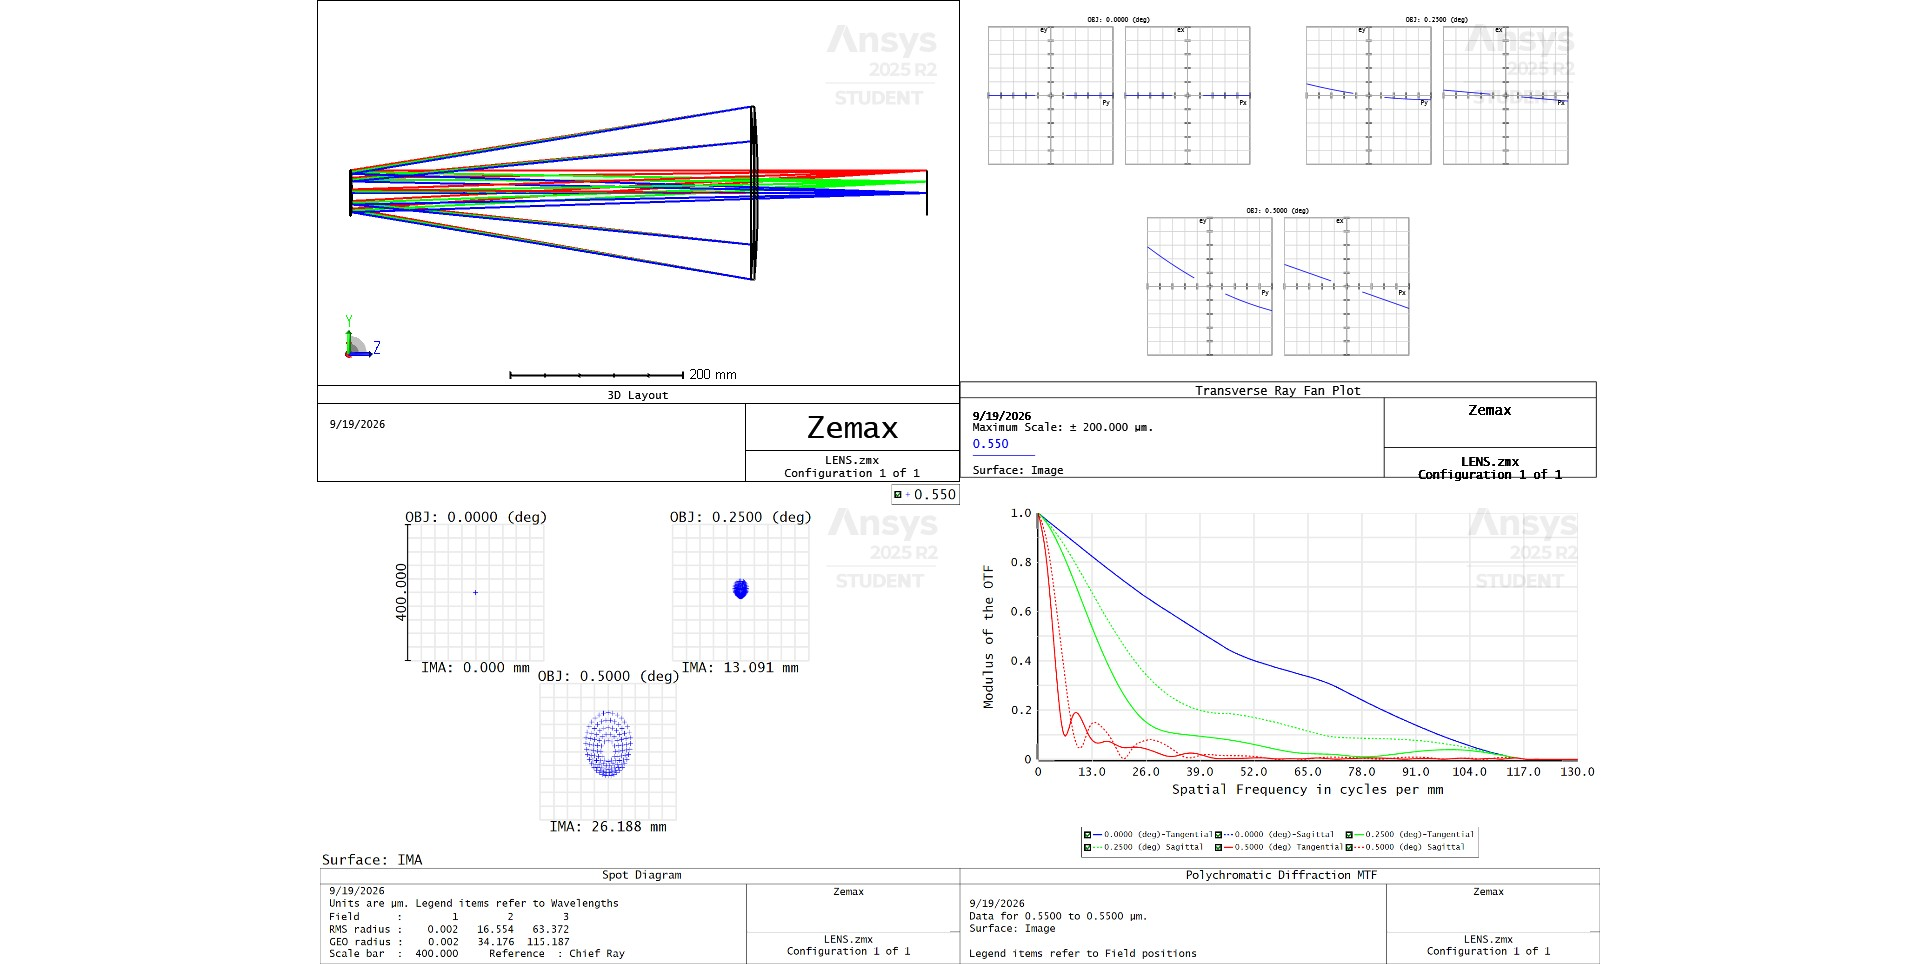
\includegraphics[width=\textwidth]{02/cassegrain_report.jpg}
\caption{Classical Cassegrain, $f/15$. The on-axis spot is a point; the
off-axis spots grow quadratically with the field angle.}
\label{fig:cass}
\end{figure*}



\subsection{Lenses}
\label{sec:res-lens}

Two N-BK7 singlets were traced, an equi-biconvex at $f/5$ and a plano-convex
at $f/2.5$ (Table~\ref{tab:lenses}, Fig.~\ref{fig:equibi}). Their on-axis RMS
radii, \SI{478}{} and \SI{860}{\micro\meter}, are two orders of magnitude
above the Airy radius, and the spot barely changes between the on-axis and
the \SI{1}{\degree} field, which shows the residual is spherical aberration
and not a field aberration. Compared with the spherical mirror of the same
focal ratio the singlet is between four and seven times worse, and it also
carries the chromatic spread of the three wavelengths, absent in every mirror
system.

\begin{table}[htbp]
\caption{N-BK7 singlets of \SI{200}{\milli\meter} aperture, traced at 450,
550 and \SI{650}{\nano\meter}. Radii in \si{\micro\meter}.}
\label{tab:lenses}
\centering
\small
\begin{tabular}{@{}lccccc@{}}
\toprule
\textbf{Shape} & $N$ & RMS $0^\circ$ & Max $0^\circ$ &
RMS \SI{1}{\degree} & Mirror, same $N$ \\
\midrule
Equi-biconvex & 4.9  & 478.3 & 1106 & 426.0 & 71.9 \\
Plano-convex  & 2.44 & 860.3 & 1903 & 702.4 & 201.9 \\
\bottomrule
\end{tabular}
\end{table}

\begin{figure*}[tbp]
\centering
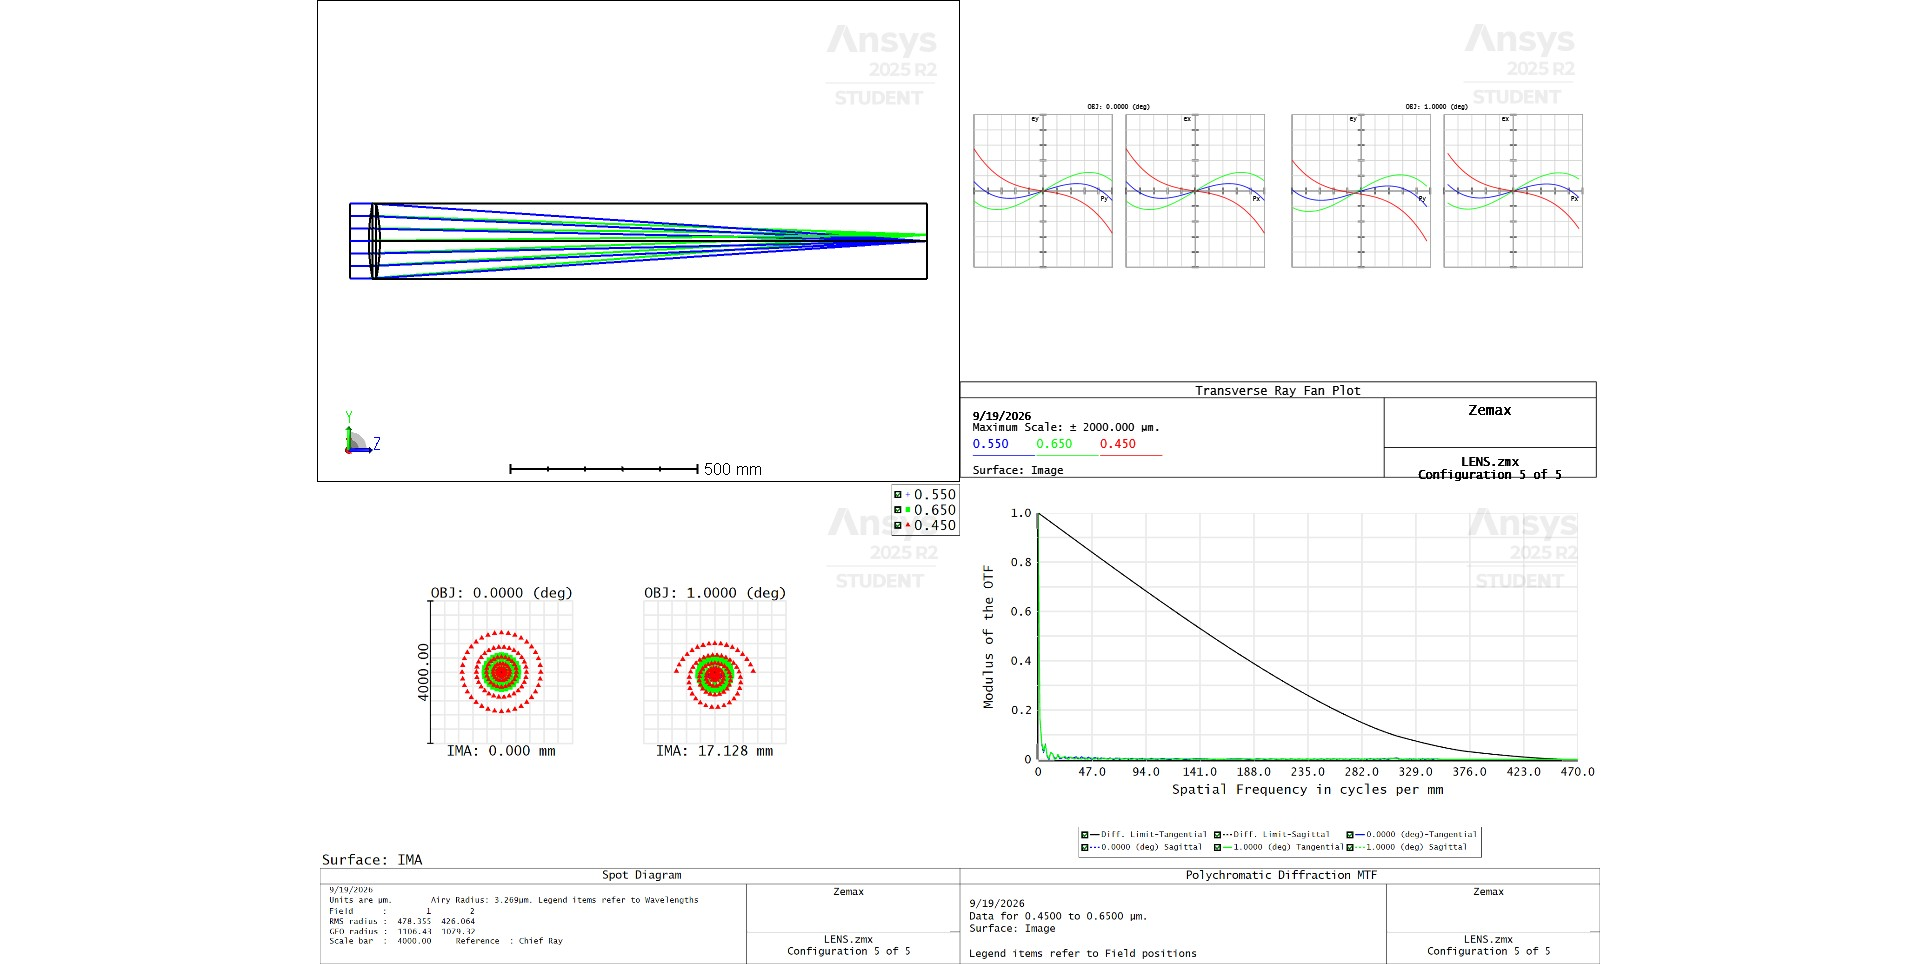
\includegraphics[width=\textwidth]{03/equibi_report.jpg}
\caption{Equi-biconvex N-BK7 singlet. The three wavelengths separate both in
the ray fan and in the spot diagram, and the MTF is close to zero over almost
the whole frequency range.}
\label{fig:equibi}
\end{figure*}

\section{Discussion}
\label{sec:disc}

\subsection{Mirrors}

The paraboloid removes
spherical aberration exactly and at every focal ratio, but leaves the field
untouched, exactly as \eqref{eq:osc} predicts since coma does not depend on
$K$. The sphere is the opposite case: its defect is entirely on axis and
disappears on its own as the focal ratio grows, because $W_{PV}$ falls as
$N^{-3}$. Past $f/15$ the two surfaces are equivalent for practical purposes,
which is the reason spherical mirrors are still used.

\subsection{Telescopes}

Nulling spherical aberration is achieved by all four designs and is therefore
not a discriminant. What separates them is the field, and the ordering is not
the expected one: the Newtonian is five times better at \SI{0.5}{\degree}
than the two Cassegrain-type designs. The reason is that the Newtonian is a
single slow $f/15$ surface, while the others fold a fast $f/3$ primary whose
field aberrations the secondary amplifies. The Newtonian pays for it with a
three-metre tube against \SI{467}{\milli\meter}, and the Gregorian pays for
its flatter field with an \SI{800}{\milli\meter} tube and a
\SI{33}{\percent} obstruction.

The Ritchey-Chr\'etien does not improve the RMS radius over the classical
Cassegrain, which at first sight contradicts its purpose. It does not: at
\SI{0.5}{\degree} the dominant aberration is already astigmatism, which the
extra conic constant does not touch. The evidence is the scaling, since the
RMS grows by a factor of four between \SI{0.25}{} and \SI{0.5}{\degree},
which is the $\beta^2$ law of astigmatism and not the $\beta$ law of coma.
The coma that the Ritchey-Chr\'etien does remove appears in the maximum
radius, \SI{16}{\percent} smaller, because it is the asymmetric tail of the
patch and not its overall size.

\subsection{Lenses}

The singlets are the worst systems measured, between four and seven times
worse than a mirror of the same focal ratio and with a chromatic spread on
top of it. Both defects come from the same place: refraction depends on the
index, which is both strongly curvature-dependent and wavelength-dependent,
whereas reflection is neither. This is the quantitative reason why every
large astronomical telescope is a reflector.

\section{Conclusions}
\label{sec:concl}

Spherical aberration is a solved problem in two independent ways: by
aspherizing the surface, which works at any focal ratio, or by making the
system slow enough, since the wavefront error falls as $N^{-3}$ and the
$f/20$ sphere is already diffraction limited. Neither solution helps off
axis.

Among the telescopes the field, not the axis, is what separates the designs,
and the aberration that limits them at \SI{0.5}{\degree} is astigmatism
rather than coma. That is why the Ritchey-Chr\'etien shows its advantage only
in the shape of the patch, and why the slow single-mirror Newtonian, at the
cost of a tube six times longer, outperforms all the folded designs.

The main limitation of this analysis is that the two singlets were traced at
different focal ratios, so the effect of the lens shape could not be isolated
from the effect of $N$; repeating both shapes at a common focal ratio, and
adding the achromatic doublet, would complete the refracting section.

\begin{thebibliography}{1}

\bibitem{guide}
L. Vanzi, \emph{Optical Aberrations} and \emph{Computer Analysis and Design of
Optical Systems for Astronomy}, course notes IEE3873, Pontificia Universidad
Cat\'olica de Chile.

\bibitem{atmos}
M. Riccardi, \emph{ATMOS -- Optical Design and Analysis Software}, v8.96.
\url{https://www.atmos-software.it}

\bibitem{schroeder}
D. J. Schroeder, \emph{Astronomical Optics}, 2nd ed. San Diego, CA: Academic
Press, 2000.

\end{thebibliography}

\end{document}
